\newthought{\textbf{Adjie Yusmunandar - 2020903430005 - TRKJ 3B}}


\newday{\textbf{1 - 2 Desember 2022} - Instalasi dan Konfigurasi Apache Hadoop}
\begin{enumerate}
\item Kendala dan Solusi \\
Kendala :\\
Saat melakukan penginstalan hadoop terdapat masalah pada saat mengecek hadoop version dan  pada saat melakukan konfigurasi hadoop terdapat kendala pada saat melakukan hdfs namenode -format. Perintah ini tidak mau dijalankan karena ada kesalahan dalam penulisan pada file yarn-site.xml.

Solusi :\\
Melakukan perubahan penulisan pada file yarn-site.xml,

\item Kesimpulan
\newline
 penginstalan hadoop dan konfigurasi hadoop berhasil dijalankan sesuai perintah-perintah yang ada.

\begin{figure}
\setlength{\belowcaptionskip}{-10pt}
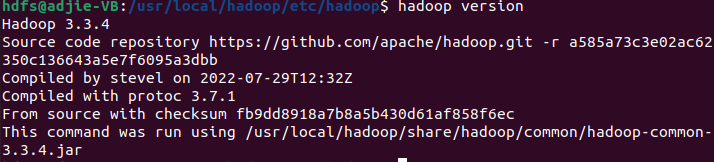
\includegraphics[width=\textwidth]{Adjie Yusmunandar/instalasi hadoop}
\caption{Versi hadoop yang Terinstall}
\label{gam:hasil instalasi apache hadoop}
\end{figure}

\begin{figure}
\setlength{\belowcaptionskip}{-10pt}
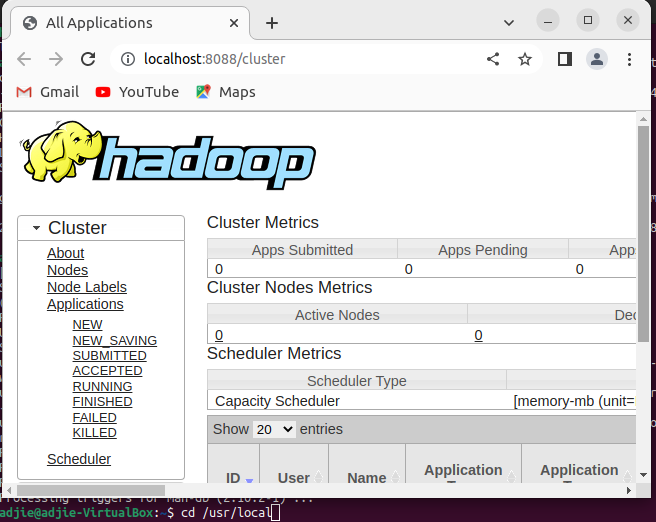
\includegraphics[width=\textwidth]{Adjie Yusmunandar/Hasil dari localhost 8080}
\caption{Hasil dari localhost 8080}
\label{gam:hasil konfigurasi hadoop}
\end{figure}

\begin{figure}
\setlength{\belowcaptionskip}{-10pt}
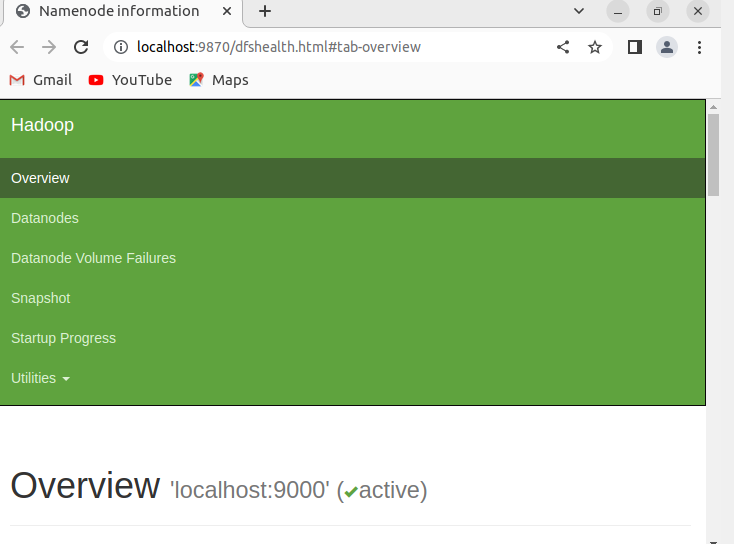
\includegraphics[width=\textwidth]{Adjie Yusmunandar/Hasil dari localhost 9870}
\caption{Hasil dari localhost 9870}
\label{gam:hasil konfigurasi hadoop}
\end{figure}
\end{enumerate}

\newday{\textbf{15 Desember 2022} - WordCount Bawaan Hadoop}
\begin{enumerate}
\item Kendala dan Solusi \\
Pada pertemuan hari ini, kegiatan yang dilakukan adalah mencoba program bawaan Hadoop untuk memahami bagaimana
proses dan cara kerja Hadoop dalam memproses data input hingga menghasilkan sebuah output. Selama praktikum tidak mengalami kendala.

\item Kesimpulan\\
Berhasil mencoba program bawaan Hadoop yaitu program menghitung jumlah kata dalam data input yang diberikan.Berikut ini gambar bukti keberhasilan praktikum. 

\begin{figure}
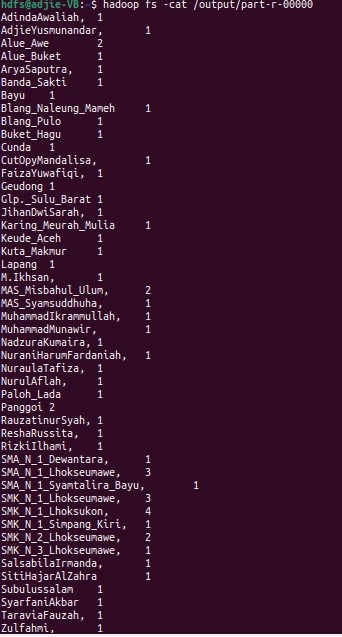
\includegraphics[width=\textwidth]{Adjie Yusmunandar/hasill wordcount bawaan hadoop}
\caption{Output Wordcount Bawaan Hadoop}
\label{gam:WordCount bawaan-Hadoop}
\end{figure}

\end{enumerate}

\newday{\textbf{22 Desember 2022} - Instalasi Apache Spark (PySpark)}
\begin{enumerate}
\item Kendala dan Solusi \\
% jelaskan kendala dan penyebab yang dialami saat mengikuti praktikum serta solusi atau langkah-langkah yang telah dilakukan
Tidak ada kendala disaat menginstall.

\item Kesimpulan\\
% berikan kesimpulan dari praktikum yang telah dikerjkan
Berhasil melakukan instalasi apache spark (PySpark), berikut hasil praktikum :

\begin{figure}
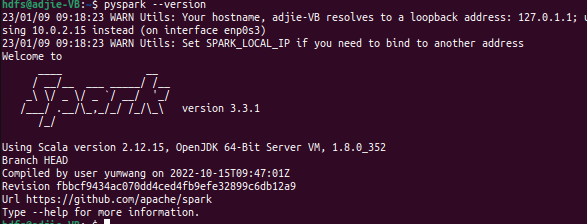
\includegraphics[width=\textwidth]{Adjie Yusmunandar/Instalasi Apache Spark}
\caption{Hasil dari localhost 9870}
\label{gam:hasil konfigurasi hadoop}
\end{figure}
\end{enumerate}